\documentclass[journal]{vgtc}                % final (journal style)
%\documentclass[review,journal]{vgtc}         % review (journal style)
%\documentclass[widereview]{vgtc}             % wide-spaced review
%\documentclass[preprint,journal]{vgtc}       % preprint (journal style)
%\documentclass[electronic,journal]{vgtc}     % electronic version, journal

%% Uncomment one of the lines above depending on where your paper is
%% in the conference process. ``review'' and ``widereview'' are for review
%% submission, ``preprint'' is for pre-publication, and the final version
%% doesn't use a specific qualifier. Further, ``electronic'' includes
%% hyperreferences for more convenient online viewing.

%% Please use one of the ``review'' options in combination with the
%% assigned online id (see below) ONLY if your paper uses a double blind
%% review process. Some conferences, like IEEE Vis and InfoVis, have NOT
%% in the past.

%% Please note that the use of figures other than the optional teaser is not permitted on the first page
%% of the journal version.  Figures should begin on the second page and be
%% in CMYK or Grey scale format, otherwise, colour shifting may occur
%% during the printing process.  Papers submitted with figures other than the optional teaser on the
%% first page will be refused.

%% These three lines bring in essential packages: ``mathptmx'' for Type 1
%% typefaces, ``graphicx'' for inclusion of EPS figures. and ``times''
%% for proper handling of the times font family.

\usepackage{mathptmx}
\usepackage{graphicx}
\usepackage{times}
\usepackage{epstopdf}
\usepackage{float}

%% We encourage the use of mathptmx for consistent usage of times font
%% throughout the proceedings. However, if you encounter conflicts
%% with other math-related packages, you may want to disable it.

%% This turns references into clickable hyperlinks.
\usepackage[bookmarks,backref=true,linkcolor=black]{hyperref} %,colorlinks
\hypersetup{
  pdfauthor = {},
  pdftitle = {},
  pdfsubject = {},
  pdfkeywords = {},
  colorlinks=true,
  linkcolor= black,
  citecolor= black,
  pageanchor=true,
  urlcolor = black,
  plainpages = false,
  linktocpage
}

%% If you are submitting a paper to a conference for review with a double
%% blind reviewing process, please replace the value ``0'' below with your
%% OnlineID. Otherwise, you may safely leave it at ``0''.
\onlineid{0}

%% declare the category of your paper, only shown in review mode
\vgtccategory{Research}

%% allow for this line if you want the electronic option to work properly
\vgtcinsertpkg

%% In preprint mode you may define your own headline.
%\preprinttext{To appear in IEEE Transactions on Visualization and Computer Graphics.}

%% Paper title.

\title{CS519: Visualization of software streamlines}

%% This is how authors are specified in the journal style

%% indicate IEEE Member or Student Member in form indicated below
\author{Sergii Shmarkatiuk}
\authorfooter{
%% insert punctuation at end of each item
\item
 Sergii Shmarkatiuk is a PhD student at Oregon State University. E-mail: shmarkas@eecs.oregonstate.edu
}

%other entries to be set up for journal
\shortauthortitle{S. Shmarkatiuk \MakeLowercase{\textit{et al.}}: Visualization of software streamlines}
%\shortauthortitle{Firstauthor \MakeLowercase{\textit{et al.}}: Paper Title}

%% Abstract section.
\abstract{Visualization of software streamlines is a first step towards a visualization technique that enables software engineers, release engineers and researchers to explore and analyze relationships between software versions. Representation of software streamlines is a very powerful way to visualize software history. It is possible to incorporate up to 14 different properties, metrics or relationships into software streamline representation, such as time, version numbers, version patterns, Version Control System artifacts, streamline types and many others. } % end of abstract

%% Keywords that describe your work. Will show as 'Index Terms' in journal
%% please capitalize first letter and insert punctuation after last keyword
\keywords{Visualization, software history, software maintenance, software configuration management, release management}

%% ACM Computing Classification System (CCS). 
%% See <http://www.acm.org/class/1998/> for details.
%% The ``\CCScat'' command takes four arguments.

%\CCScatlist{ % not used in journal version
% \CCScat{K.6.1}{Management of Computing and Information Systems}%
%{Project and People Management}{Life Cycle};
% \CCScat{K.7.m}{The Computing Profession}{Miscellaneous}{Ethics}
%}

%% Uncomment below to include a teaser figure.
%   \teaser{
%   \centering
%   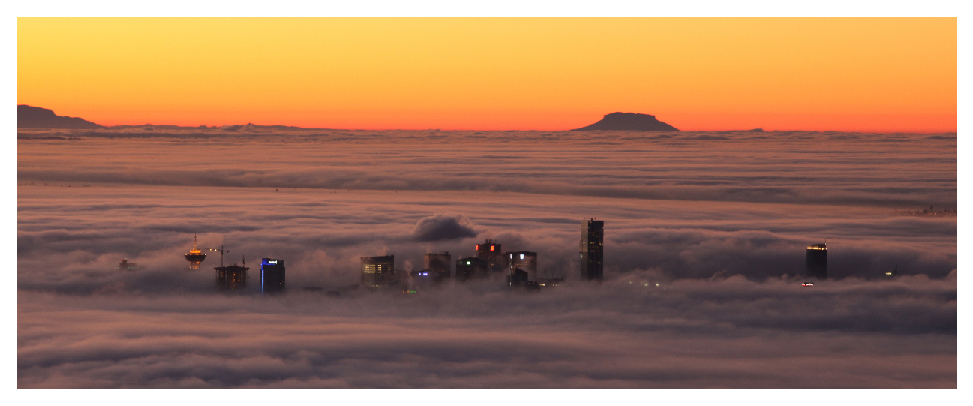
\includegraphics[width=16cm]{CypressView}
%   \caption{In the Clouds: Vancouver from Cypress Mountain.}
%  }

%% Uncomment below to disable the manuscript note
%\renewcommand{\manuscriptnotetxt}{}

%% Copyright space is enabled by default as required by guidelines.
%% It is disabled by the 'review' option or via the following command:
% \nocopyrightspace

%%%%%%%%%%%%%%%%%%%%%%%%%%%%%%%%%%%%%%%%%%%%%%%%%%%%%%%%%%%%%%%%
%%%%%%%%%%%%%%%%%%%%%% START OF THE PAPER %%%%%%%%%%%%%%%%%%%%%%
%%%%%%%%%%%%%%%%%%%%%%%%%%%%%%%%%%%%%%%%%%%%%%%%%%%%%%%%%%%%%%%%%

\begin{document}

%% The ``\maketitle'' command must be the first command after the
%% ``\begin{document}'' command. It prepares and prints the title block.

%% the only exception to this rule is the \firstsection command
\firstsection{Introduction}

\maketitle

%% \section{Introduction} %for journal use above \firstsection{..} instead
Primary target audience of software streamlines visualization is release engineers. Release engineers will find beneficial to use visualization of software streamlines to: 
\begin{itemize}
\item Track history of software applications
\item Analyze and control complexity of software projects
\item Allocate resources for support of existing and future version of software applications
\item Manage infrastructure and deployments of software versions to target environments
\end{itemize}
We expect that software streamlines visualization will also be useful for software engineers, software testing engineers, quality assurance/process engineers, support engineers, project managers and researchers.

\section{Questions from users}
There are several categories of streamline visualization users that might ask different kind of questions about data:

\paragraph{Release engineers}
	\begin{enumerate}
		\item \textbf{Frequency.} How often does software development team produce new version of software application? 
		\item \textbf{Team.} How many developers work on different parts/branches/streamlines of software application? Correlates with previous question and helps to predict how often new version of software application is getting released from different branches/streamlines.
		\item \textbf{Source code.} How much source code (LOC, size of diffs between versions) does software application contain? Answer to this question might help to predict how long it usually takes to build/rebuild application from scratch and deploy it to the target platform. Which, in turn, helps with calculation of ETA for releases and deployments of software applications.
		\item \textbf{Deployments.} What are the most recently released/deployed versions of software application? What are the platforms where application is deployed? What are the recent/upcoming versions of software applications that require deployment? 
	\end{enumerate}

\paragraph{Software engineers}
\begin{enumerate}
	\item \textbf{Context.} What am I currently working on? I want to see the version of software application I am currently working on and how it is related to other (past, future, similar) versions of the same application.
	\item \textbf{Bugfixes.} I want to fix bug in version a.b.c. What is the branch/streamline I should work on to get rid of the bug in the majority of other versions of the same software application? I fixed bug in version a.b.c. Where else should I fix it? 
	\item \textbf{Source code changes.} What kinds of changes am I allowed to perform in certain branches? What is the most appropriate place (branch/streamline) for my change?
	\item \textbf{Compatibility.} Where do I need to reimplement existing feature from scratch due to restrictions of versions compatibility?
\end{enumerate}

\paragraph{Software testing engineers}
	\begin{enumerate}
		\item \textbf{Bugs.} I found bug x in version a.b.c. What other versions should I test in order to find the same bug or similar bugs? What is the version of software application where bug x appeared first? When I report bug, what versions should I mention? 
		\item \textbf{Features.} I don’t want to spend unnecessary effort testing feature x and creating erroneous bug-reports related to this feature. I want to know when and where (version) did feature x appear first time?
	\end{enumerate}
	
\paragraph{Project managers, quality assurance and process engineers}
	\begin{enumerate}
		\item \textbf{Quality.} How many bugs do different versions of software application usually have? What is the threshold of allowed number of bugs for different versions? Do number of bugs and their severity depend on type and maturity level of artifact where they were found?
		\item \textbf{Process.} What are the bottlenecks in the process? When does it take more time to release next version of software application?  When is it appropriate to introduce specific practice to improve software development process (for example, will practice of static analysis be more effective for development streamlines or release streamlines based on frequency of software builds/releases?)
	\end{enumerate}

\paragraph{Researchers}
	\begin{enumerate}
		\item \textbf{Statistics.} How do such metrics as number of developers, lines of source code and methodologies affect speed, quality and cost of development? 
		\item \textbf{Prediction.} Estimate probability of certain events (problems with compatibility, spending more time for software delivery than initially estimated) happening based on historical data. 
		\item \textbf{Theories.} Investigating correlation between different metrics to come up with new hypotheses about software evolution. Investigating how conclusions generalize for different cases by comparing visualizations for different versions of software.
	\end{enumerate}

\section{Data}
\subsection{Data variables}

\begin{table}[H]
%% Table captions on top in journal version
 \scriptsize
 \begin{center}
   \begin{tabular}{|l|c|p{3cm}|} 
   \hline
     \textbf{Variable} & \textbf{Type} & \textbf{Values} \\
   \hline
   \hline
     Version numbers  & numeric/ordinal & 1.x.0, 1.x.1, 2.3.45, x.8.12, ... \\ \hline  
     Maturity levels & ordinal & Development, Testing, User acceptance, Release Candidate, Stable \\ \hline  
     Timestamps & numeric & 1398587257, 1398586400, 1398298452, ... \\ \hline  
     Version Control System artifacts & nominal & portingToX64, HibernateIntegration, prototypeImplementation, ... \\ \hline  
     Streamline types & nominal & mainline, support, release, experimental \\ \hline  
     Lines of source code & numeric & 589, 1045, 78563, ... \\ \hline  
     Size of development team & numeric & 5, 10, 30, ... \\ \hline  
     Deployment platforms & nominal & test.company.com, dev.company.com, ci.company.com, ... \\ \hline  
     Number of deployed applications & numeric & 5, 10, 30, ... \\ \hline  
     
   \end{tabular}
   \caption{Data variables}
   \label{data_variables}
\end{center}
\end{table}

%\begin{figure}[htb]
% \centering
% 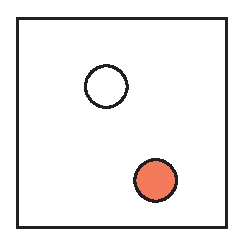
\includegraphics[width=1.5in]{sample}
% \caption{Sample illustration.}
%\end{figure}

\subsection{Abstract operations}

%% TODO:

\subsection{Data type abstractions}

%% TODO:

\subsection{Encodings}

%% TODO:


\section{Conclusion}

Lorem ipsum dolor sit amet, consetetur sadipscing elitr, sed diam
nonumy eirmod tempor invidunt ut labore et dolore magna aliquyam erat,
sed diam voluptua. At vero eos et accusam et justo duo dolores et ea
rebum. Stet clita kasd gubergren, no sea takimata sanctus est Lorem
ipsum dolor sit amet. Lorem ipsum dolor sit amet, consetetur
sadipscing elitr, sed diam nonumy eirmod tempor invidunt ut labore et
dolore magna aliquyam erat, sed diam voluptua. At vero eos et accusam
et justo duo dolores et ea rebum. Stet clita kasd gubergren, no sea
takimata sanctus est Lorem ipsum dolor sit amet. Lorem ipsum dolor sit
amet, consetetur sadipscing elitr, sed diam nonumy eirmod tempor
invidunt ut labore et dolore magna aliquyam erat, sed diam
voluptua. At vero eos et accusam et justo duo dolores et ea
rebum. Stet clita kasd gubergren, no sea takimata sanctus est Lorem
ipsum dolor sit amet.

Lorem ipsum dolor sit amet, consetetur sadipscing elitr, sed diam
nonumy eirmod tempor invidunt ut labore et dolore magna aliquyam erat,
sed diam voluptua. At vero eos et accusam et justo duo dolores et ea
rebum. Stet clita kasd gubergren, no sea takimata sanctus est Lorem
ipsum dolor sit amet. Lorem ipsum dolor sit amet, consetetur
sadipscing elitr, sed diam nonumy eirmod tempor invidunt ut labore et
dolore magna aliquyam erat, sed diam voluptua. At vero eos et accusam
et justo duo dolores et ea rebum. 

%% if specified like this the section will be committed in review mode
% \acknowledgments{
% The authors wish to thank A, B, C. This work was supported in part by
% a grant from XYZ.}

\bibliographystyle{abbrv}
%%use following if all content of bibtex file should be shown
%\nocite{*}
\bibliography{template}
\end{document}

